\documentclass[10pt,a4paper]{article}
\usepackage{amsmath}
\usepackage{amsfonts}
\usepackage{amssymb}
\usepackage{graphicx}
\usepackage[french]{babel}
\usepackage[T1]{fontenc}
\usepackage[utf8x]{inputenc}
\graphicspath{{images/}}
\usepackage{parskip}
\usepackage{fancyhdr}
\usepackage{vmargin}
\usepackage{caption}
\usepackage{subcaption}
\setmarginsrb{3 cm}{2.5 cm}{3 cm}{2.5 cm}{1 cm}{1.5 cm}{1 cm}{1.5 cm}

\title{Assistance pour les patients atteints de la maladie d'Alzheimer}                             % Title
\author{Maxime De Wolf\\
		Dimitri Waelkens}                               % Author
\date{\today}                                           % Date

\makeatletter
\let\thetitle\@title
\let\theauthor\@author
\let\thedate\@date
\makeatother

\pagestyle{fancy}
\fancyhf{}
\rhead{\theauthor}
\lhead{\thetitle}
\cfoot{\thepage}

\begin{document}
   	
   	%%%%%%%%%%%%%%%%%%%%%%%%%%%%%%%%%%%%%%%%%%%%%%%%%%%%%%%%%%%%%%%%%%%%%%%%%%%%%%%%%%%%%%%%%
   	
   	\begin{titlepage}
   		\centering
   		\vspace*{0.5 cm}
   		
\includegraphics[scale = 0.75]{UMONS}\\[1.0 cm]   % University Logo
   		\textsc{\LARGE Université de Mons}\\[2.0 cm]   % University Name
   		\textsc{\large Défi en en Intelligence Artificielle}\\[0.5 cm]               % Course Name
   		\rule{\linewidth}{0.2 mm} \\[0.4 cm]
   		{ \huge \bfseries \thetitle}\\
   		\rule{\linewidth}{0.2 mm} \\[1.5 cm]
   		
   		\begin{minipage}{0.4\textwidth}
   			\begin{flushleft} \large
   				\emph{Auteur:}\\
   				\theauthor
   			\end{flushleft}
   		\end{minipage}~
   		\begin{minipage}{0.4\textwidth}
   			\begin{flushright} \large
   				\emph{Dimitri Waelkens}                                  % Your Student Number
   			\end{flushright}
   		\end{minipage}\\[2 cm]
   		
   		{\large \thedate}\\[2 cm]
   		
   		\vfill
   		
   	\end{titlepage}
   	
   	\section{Objectif}
   	
   		Dans le cadre du cours de \textit{Défi en Intelligence Artificielle}, il nous a été demandé d'entraîner un réseau de neurones afin de pouvoir localiser des clés à partir d'images. Cela a pour finalité d'aider les personnes touchées par la maladie d'Alzheimer à retrouver leurs clés dans leur domicile grâce à divers caméras disposées dans l'habitation. Cette technique peut être appliquée à d'autres objets pour fournir une assistance complète à ces personnes.\\
   		
   		Dans ce rapport, nous commençons détailler la manière dont nous avons obtenu notre \textit{dataset}. Ensuite, nous présentons nos résultats obtenus grâce à \textbf{YOLO V3}. Nous concluons ce rapport en abordant la manière dont nous aurions pû améliorer nos résultats. 
   	
   	\section{Obtention du \textit{dataset}}
   	
   		La première partie est très importante car il s'agit de la collecte du \textit{dataset}. En effet, le \textit{dataset} a pour but d'entraîner notre réseaux de neurones. Il est donc primordial que celui-ci soit de bonne qualité pour que notre réseau soit performant. De plus, il faut également qu'il soit assez bien fourni pour éviter que les données d'entraînement ne biaise notre réseau.\\
   		
   		Malheureusement, aucun \textit{dataset} relatif à notre problématique n'est disponible sur Internet. Il a donc fallut le construire manuellement presque à partir de zéro. Heureusement, nous disposions initialement de quelques centaines d'images de clés annotées pour constituer notre \textit{dataset} de base.\\
   		
   		Nous avons donc dû rechercher des images de clés et les annoter afin de faire grossir notre \textit{dataset}. Cette étape est fastidieuse, c'est pourquoi nous nous sommes associés à d'autres groupes afin de former un \textit{dataset} commun relativement conséquent et de bonne qualité. Nous avons ainsi réussi à récolter un total d'un peu plus de 2300 images annotées pour constituer notre \textit{dataset}.
   		
   	\newpage
   	
   	\section{Résultats \textbf{YOLO V3}}
   	
   		Malheureusement, nous n'avons pas eu réussi à lancer l'entraînement sur notre \textit{dataset}. Nous avons néanmoins réussi à entraîner un réseau sur base des images fournies par les professeurs. La Figure \ref{fig:pred} nous montre une prédiction obtenue grâce à ce réseau. Nous pouvons conclure que notre réseau de neurones est assez mauvais dans la réalisation de sa tâche.
   		
   		\begin{figure}[h]
			\begin{center}
	   			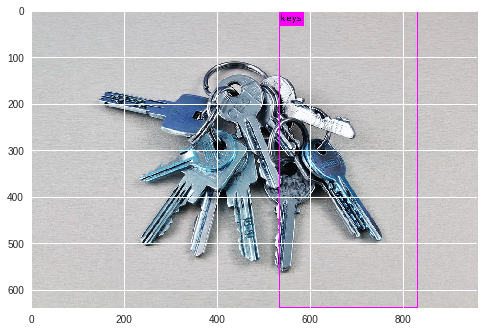
\includegraphics[width=0.5\linewidth]{pred}
	   			\caption{Prédiction de notre réseau de neurones entraînés par \textbf{YOLO V3}}
	   			\label{fig:pred}
			\end{center}
   		\end{figure}
   	
   	\section{Améliorations possibles}
   	
   		Il existe plusieurs manières qui nous permettrait d'améliorer notre réseau de neurones.   		
   		Tout d'abord, comme mentionné ci-dessus, nous ne sommes pas parvenus à entraîner notre réseau de neurones avec l'intégralité de notre \textit{dataset}. Il est évident que réseau aurait été plus performant si cela avait été le cas.\\
   		
   		Ensuite, nous aurions pû redimensionner les images de notre \textit{dataset}. En effet, certaines de ces images sont de tailles relativement importantes ce qui réduis la vitesse d'entraînement. Notre réseau aurait donc pû s'entraîner plus rapidement mais cela ne représente qu'une amélioration mineure.
   		
   		Pour finir, nous aurions pû améliorer la qualité de notre \textit{dataset}. En effet, de nombreuses images de notre \textit{dataset} représentent des gros plans de clés sans arrière-plan. Cela a tendance à biaisé l'entraînement car notre réseau à pour but de localiser des clés sur une photo d'habitation. Ces photos ne représente donc pas un échantillon pertinent pour l'entraînement. Nous nous attendons donc à un gain de performance lorsque ce problème sera réglé.
   	%\bibliographystyle{plain}
   	%\bibliography{biblist}
          	
\end{document}